\newcommand{\degree}{^{\circ}}

\chapter{Results and Discussion}

Now that we have a better understanding of how we use the Cartan frames and approximations of 1-forms in order to deduce fiber orientation at each location in the heart and computing an error of fit, we will now discuss the results obtained when applying this pipeline to different heart MRIs.

\section{Quantitative Results}

\begin{figure}
    \centering
    \begin{subfigure}{1\textwidth}
        \centering
        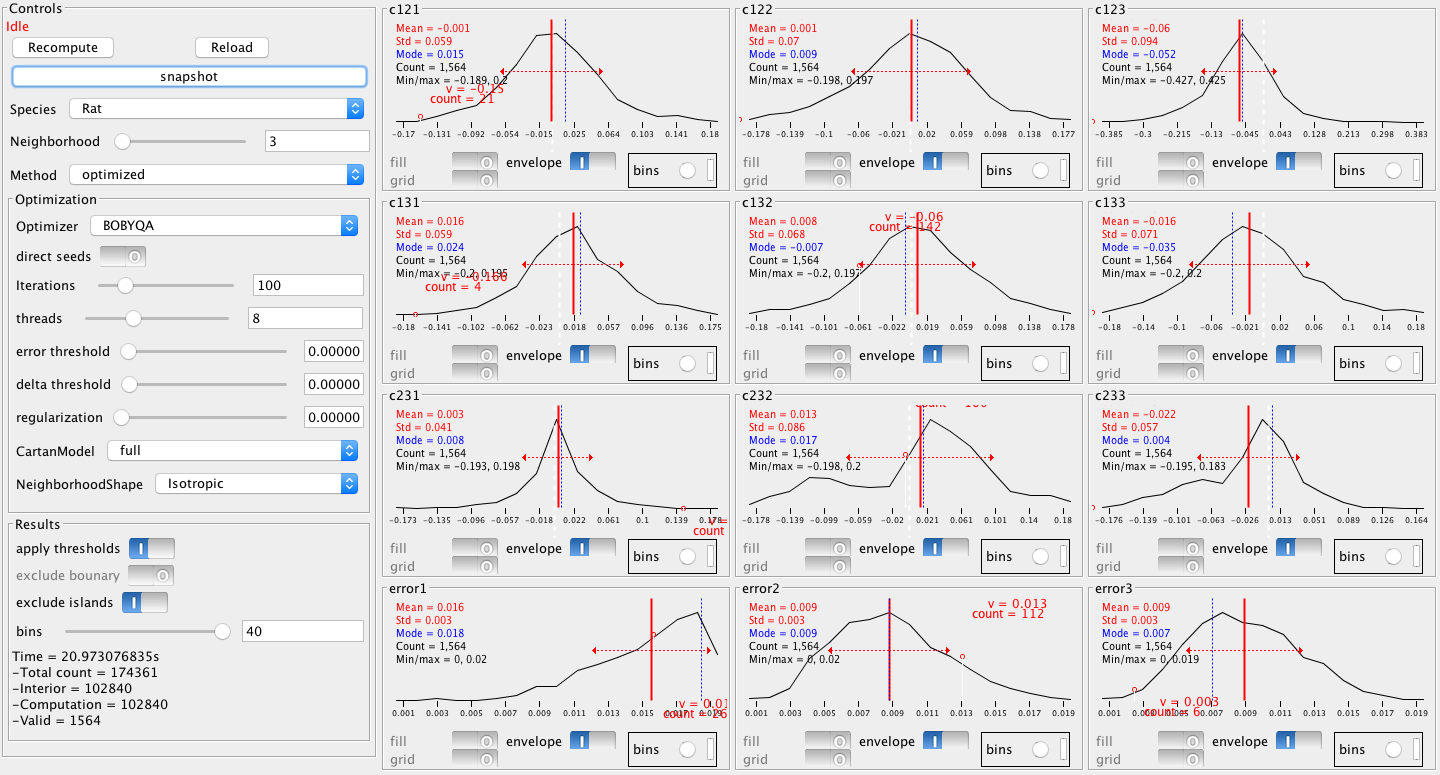
\includegraphics[width=\textwidth]{figures/histogram_pig6_no_smooth}
        \caption{Without any smoothing}
        \label{fig:histogram_pig6_no_smooth}
    \end{subfigure}
    \begin{subfigure}{1\textwidth}
        \centering
        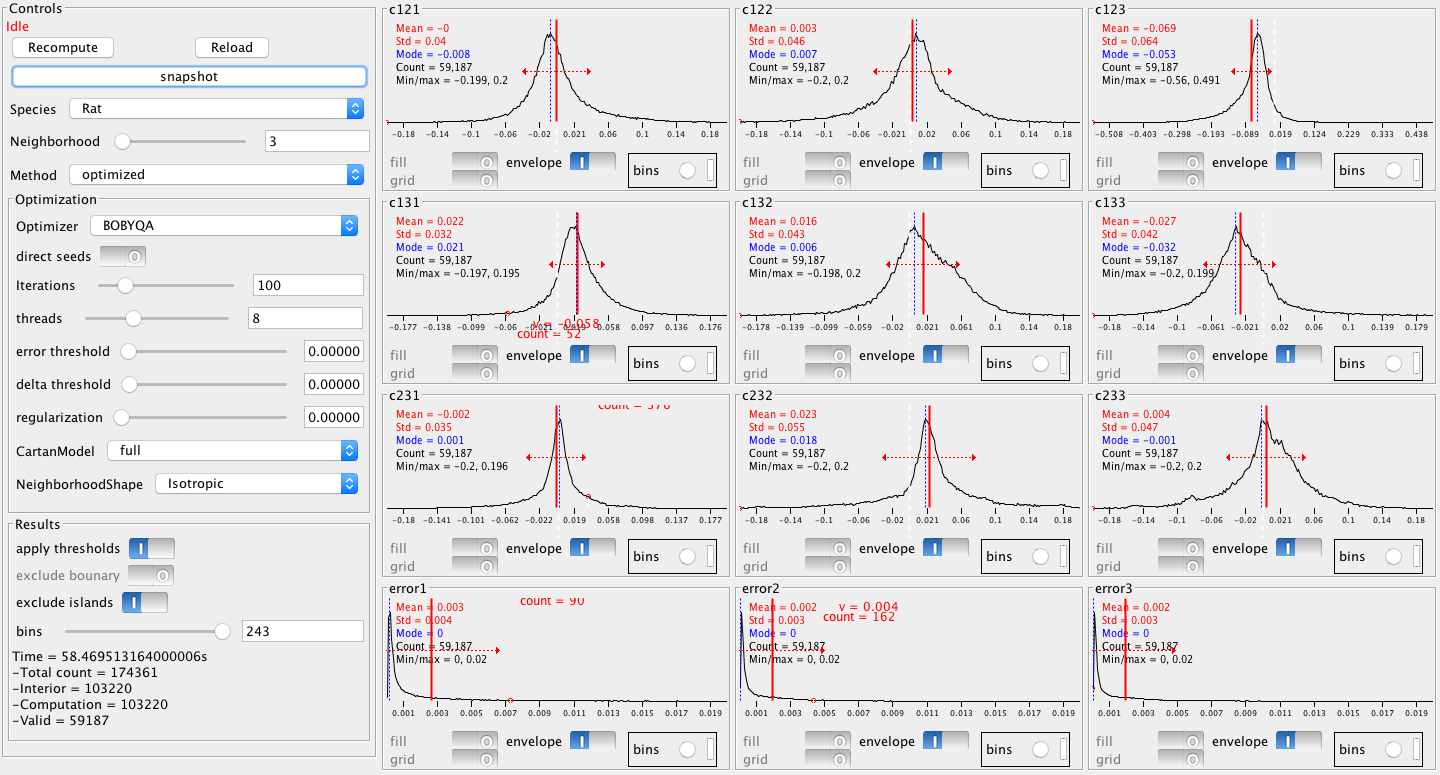
\includegraphics[width=\textwidth]{figures/histogram_pig6_smooth}
        \caption{With Rician smoothing}
        \label{fig:histogram_pig6_smooth}
    \end{subfigure}
    \caption{Histograms of error of fit and connection form parameters for pig \# 6}
    \label{histo_pig6}
\end{figure}

Given the association between ADC and our error of frame fit, it is natural to compare these measures quantitatively throughout the myocardium. We did so for the 5 infarcted porcine hearts we analyzed by computing Dice coefficients to describe the overlap, in the following manner:

For the same heart let A be the set of voxels with ADC value $> 0.6$ and let B be the set of voxels with error of fit $> 15 \degree$. We computed the standard Dice coefficient $\frac{A \cap B}{A \cup B}$ as well as a modified coefficient $\frac{A \cap B}{A}$.
\begin{table}
    \centering
    \begin{tabular}{|c | c | c |}
         \hline
         Heart & $\frac{A \cap B}{A \cup B}$ & $\frac{A \cap B}{A}$ \\
         \hline
         2 & 0.40 & 0.80 \\ 
         \hline
         4 & 0.43 & 0.89 \\
         \hline
         5 & 0.47 & 0.76 \\
         \hline
         6 & 0.46 & 0.87 \\
         \hline
         7 & 0.27 & 0.94 \\ 
         \hline
    \end{tabular}
    \caption{Dice and modified coefficients for infarcted hearts}
\end{table}

These results demonstrate that typically over 80\% of the locations with increased diffusion also yield a high error of fit using our frame fitting method, due to the loss of geometric coherence of fiber orientations. However there are additional locations where fiber orientations are not smooth, typically at the linings of the heart wall, or near the edges of a collapsing and narrow right ventricle. These are picked up by our error of fit measure but not by the ADC measure, likely because there is no increase in collagen there.

\subsection{Histograms of connection forms} \label{histogram_section}

Here are examples of the histograms that we computed on the entire heart for every usable example that we had. The histogram in Fig. \ref{fig:histogram_pig6_smooth} gives us information on the distribution of $c_{ijk}, \forall (i, j, k) \in [1, 3]^3$ and the distribution of the error of fit for each frame axis $\mathbf{f}_1, \mathbf{f}_2$ and $\mathbf{f}_3$.

In this thesis we will focus on the most commonly used parameter for comparison, the parameter related to the notion of helix angle $c_{123}$. Our tool gives us the mean and the mode (value most represented) of this value through the whole heart. Given the distribution of these values the mode is relevant since it will represent mostly fibers in the core of the heart wall but without taking into account (as the mean value does) extreme values that can occur on the boundaries of the heart wall.

The papillary muscles, to name only one anatomical structure within the heart, which are mostly aligned in a top-down direction along the long axis, can have non negligible effect on the $c_{123}$ value and they are difficult to remove from our data. These muscles are indeed difficult to remove from the data since it is not always clear which layer (in the long axis direction) they start and end in. This is why segmenting them automatically is not obvious. Moreover, thresholding the ADC value to segment tissue with oriented structure does pick up the papillary muscle since it has fibers aligned in a long axis direction.

In the table we regroup the results we obtained from all relevant datasets and analyze the total helix angle in degrees that we obtain the following way (where 57.3 is the conversion from rad to $\degree$):
\begin{equation}
    \text{orientation from outer to inner wall} = c_{123}\cdot \text{\#voxels}\cdot 57.3
\end{equation}
Although the values that we get are close to the theoretical value of $120\degree$ reported in the literature \cite{piuzephd}, there is too high variability to be able to draw conclusions from these values, but they can be helpful to understand at a bigger scale the distribution of the fiber orientations we obtained.

\begin{table}
    \centering
    \begin{tabular}{|c | c | c | c| c| c|} 
         \hline
         Heart & \shortstack{Thickness \\ (\# voxels)} & \shortstack{$c_{123}$ mean \\ rad/voxel} & \shortstack{$c_{123}$ mode \\ rad/voxel} & \shortstack{Total helix angle \\ (using mean)} & \shortstack{Helix angle \\ (using mode)}\\
         \hline
         2 & 40 & -0.066 & -0.025 & -151.2$\degree$ & -57.3$\degree$ \\ 
         \hline
         4 & 45 & -0.084 & -0.047 & -216.6$\degree$ & -121.2$\degree$ \\
         \hline
         5 & 30 & -0.048 & -0.020 & -82.5$\degree$ & -34.38$\degree$ \\
         \hline
         6 & 30 & -0.069 & -0.053 & -118.6$\degree$ & -91.1$\degree$ \\
         \hline
         7 & 45 & -0.077 & -0.053 & -198.5$\degree$ & -136.6$\degree$ \\ 
         \hline
         25 & 35 & -0.072 & -0.034 & -144.4$\degree$ & -68.2$\degree$ \\
         \hline
    \end{tabular}
    \caption{Total helix angle using our connection form parameters}
\end{table}


\section{Qualitative Results}

\subsection{Importance of Rician filtering}

In this section Figure \ref{fig:pig4_topviews}, Figure \ref{fig:pig4_helix} and Figure \ref{fig:pig4_tractos} are all representing the same heart at the same slice in the long axis direction.

The topview Figure \ref{fig:pig4_topviews} gives a general idea of how muscle fibers are wrapped around the heart wall, but it is not a good evidence of the change of orientation from outer to inner wall. The transverse view in Figure \ref{fig:pig4_helix} helps to show this counterclockwise fiber turning from outer to inner wall. These snapshots are also helpful to visualize the importance of smoothing, as they show clearly that the noise is reduced by a significant amount.

The region shown in the foreground of Figure \ref{fig:pig4_helix_no_smooth} and Figure \ref{fig:pig4_helix_smooth} is a region away from the infarct where we can see a smooth turning of fibers. This region corresponds to the top-left region of the Left Ventricle of the same slice presented in Figure \ref{fig:pig4_topview_no_smooth} and Figure \ref{fig:pig4_topview_smooth}. These figures show that fibers away from the infarct are indeed not affected and are still organized in a similar way than in a healthy heart.

\begin{figure}[!h]
    \centering
    \begin{subfigure}{.48\textwidth}
        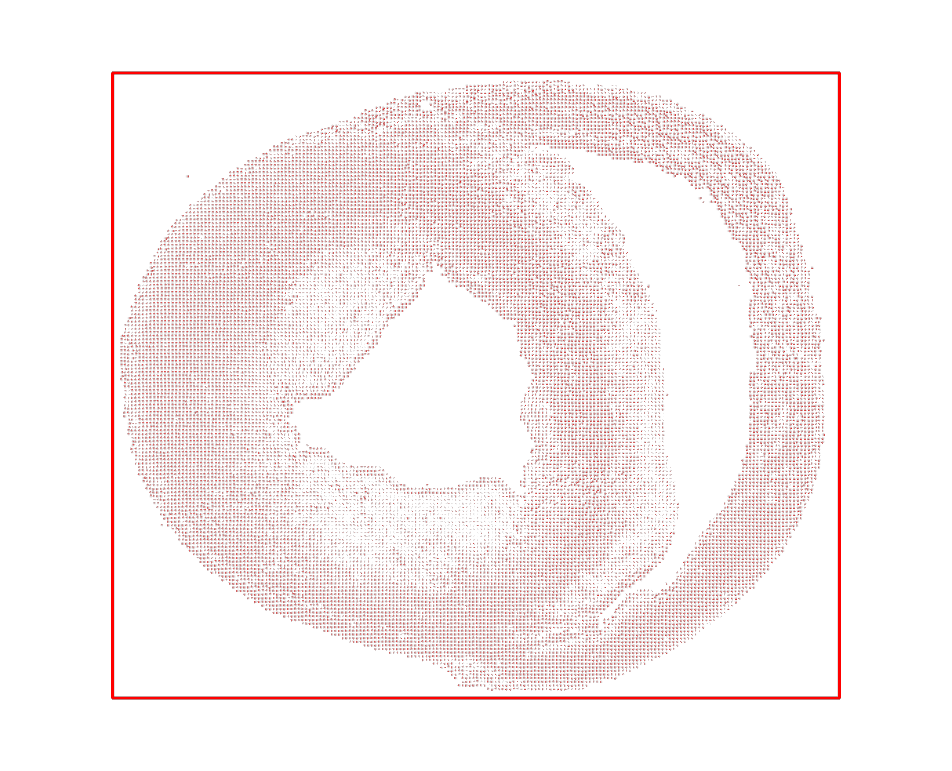
\includegraphics[width=\textwidth]{figures/pig4_topview_no_smooth}
        \caption{Without any smoothing}
        \label{fig:pig4_topview_no_smooth}
    \end{subfigure}
    \begin{subfigure}{.48\textwidth}
        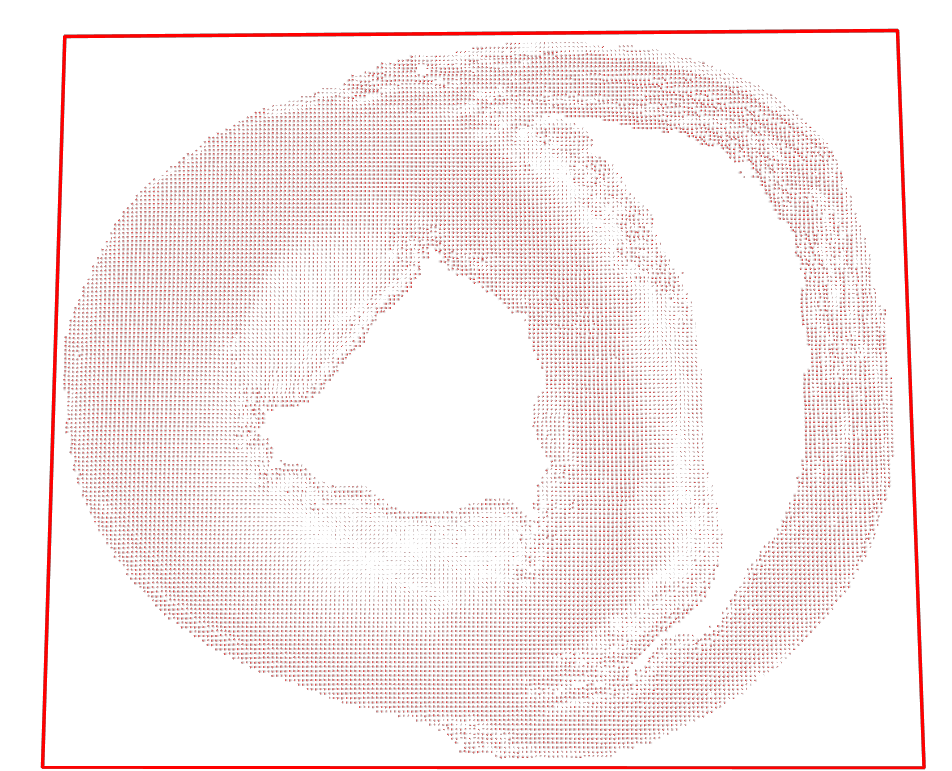
\includegraphics[width=\textwidth]{figures/pig4_topview_smooth}
        \caption{With Rician smoothing}
        \label{fig:pig4_topview_smooth}
    \end{subfigure}
    \caption{Top view of heart fibers for pig 4}
    \label{fig:pig4_topviews}
    \begin{subfigure}{.48\textwidth}
        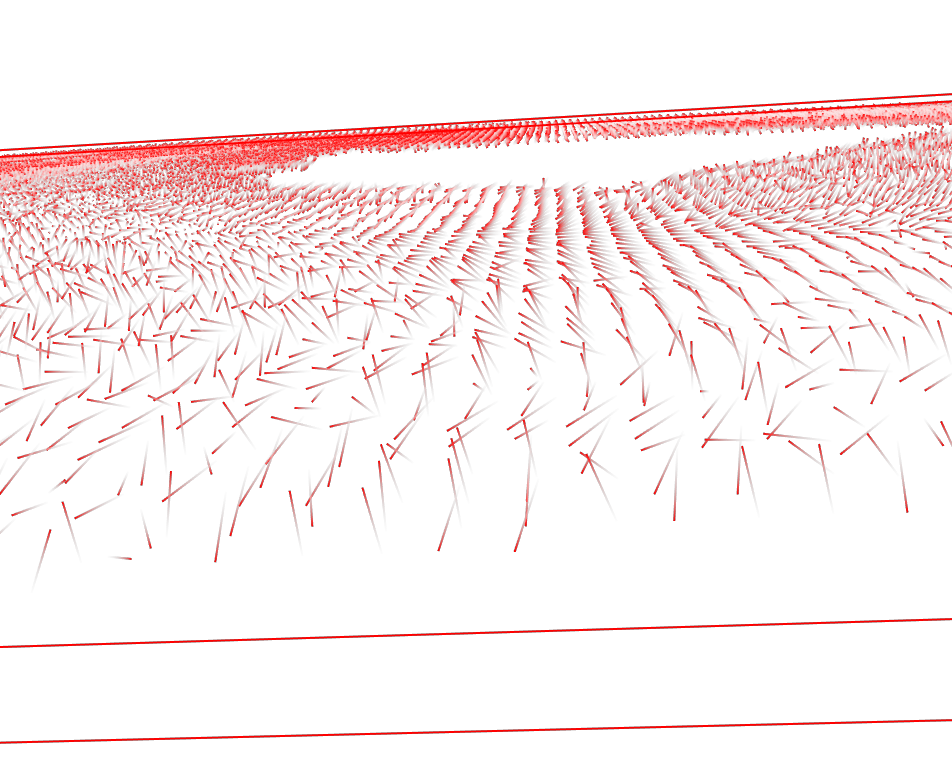
\includegraphics[width=\textwidth]{figures/pig4_helix_no_smooth}
        \caption{Without any smoothing}
        \label{fig:pig4_helix_no_smooth}
    \end{subfigure}
    \begin{subfigure}{.48\textwidth}
        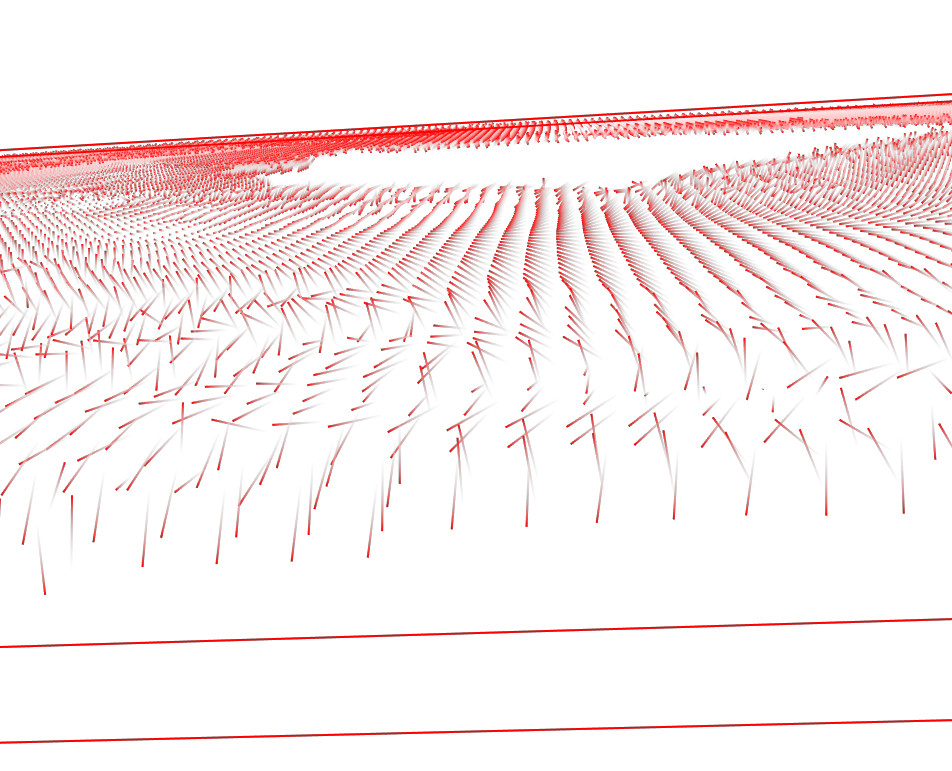
\includegraphics[width=\textwidth]{figures/pig4_helix_smooth}
        \caption{With Rician smoothing}
        \label{fig:pig4_helix_smooth}
    \end{subfigure}
    \caption{View of the helix angle of heart fibers for pig 4}
    \label{fig:pig4_helix}
\end{figure}

\subsection{Tractography and Fitting}

Using the fiber orientation that we can get from the computed tensor matrix, we can run tractography on our results. This process gives us an idea of how fibers should be wrapped around the heart and work together in the muscle structure. The way tractography works is fairly simple: the algorithm follows the direction of the fiber and when it reaches a neighbor voxel, it picks up this new direction and propagates further. The infarct region, as explained in \cite{wu2007mr}, is the region with the least coherence in its fiber directions whereas regions remote from the infarct are not be affected in their structure. The tractography is an even more obvious visualization of the regions that lack geometrical regularity. Indeed regions not affected by the infarct have their fibers wrapped smoothly along the heart wall in an organized manner.

\begin{figure}[!h]
    \centering
    \begin{subfigure}{.48\textwidth}
        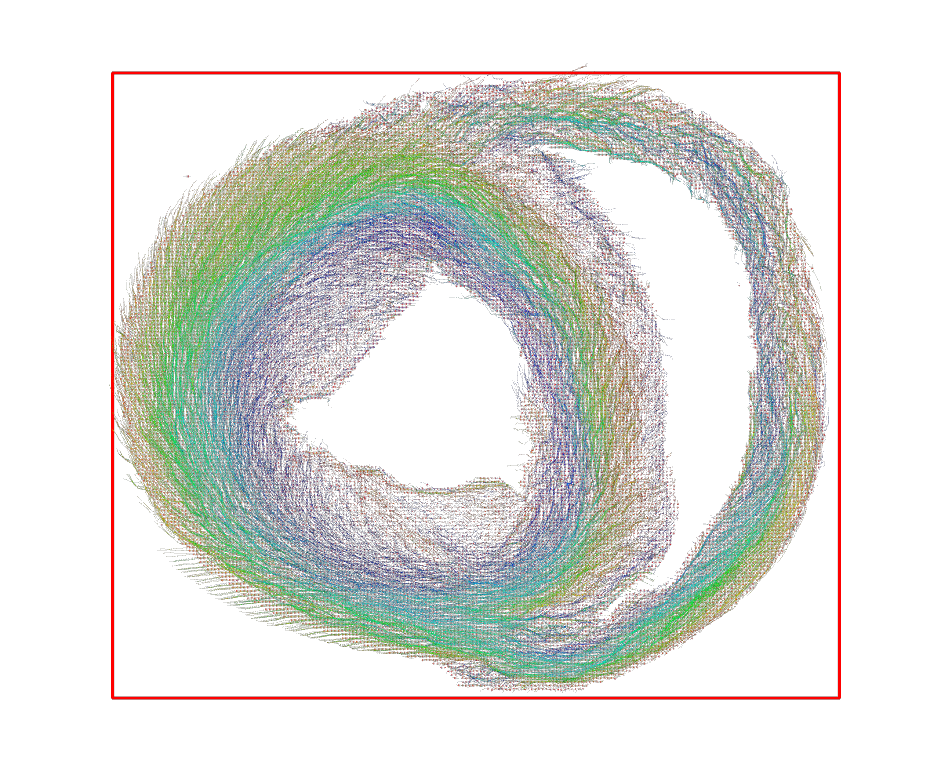
\includegraphics[width=\textwidth]{figures/pig4_topview_tracto_no_smooth}
        \caption{Without any smoothing}
        \label{fig:pig4_tracto_no_smooth}
    \end{subfigure}
    \begin{subfigure}{.48\textwidth}
        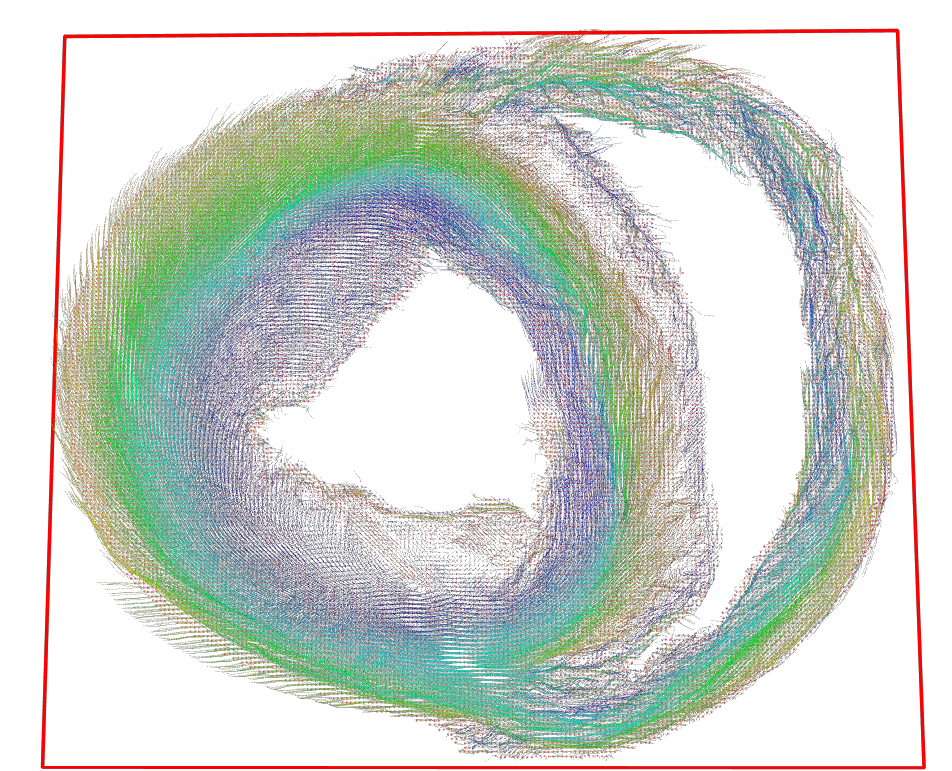
\includegraphics[width=\textwidth]{figures/pig4_topview_tracto_smooth}
        \caption{With Rician smoothing}
        \label{fig:pig4_tracto_smooth}
    \end{subfigure}
    \caption{Tractography of heart fibers for pig 4}
    \label{fig:pig4_tractos}
\end{figure}

The histograms provided in Figure \ref{fig:histogram_pig6_no_smooth} and Figure \ref{fig:histogram_pig6_smooth} give us indications on different subjects:
\begin{enumerate}
    \item With our dataset Rician smoothing is capital to be able to fit a model on the data. The algorithm was able to successfully apply the fitting method only for $1564$ voxels in the case of the unfiltered data. When Rician smoothing was applied, the algorithm could converge for $59187$ voxels, and therefore was giving us much more meaningful data on the entire heart
    \item Most fibers have their connection form parameters in the same range, and that's why most datapoints are closely centered around the mode. This is another proof showing that in the case presented here the general fiber structure of the heart was unchanged, although the deviation around the mode accounts for some irregularities in the infarct zone and close to boundaries of the inner and outer heart wall
    \item Most connection form parameters are fairly concentrated around 0, except for $c_{123}$ which accounts for the change in orientation of the fiber direction when moving from outer to inner wall
\end{enumerate}
The number of voxels that count in our computations is the number of voxels where the algorithm could converge to a value for each of the connection form parameters $(c_{ijk})_{(i, j, k) \in \mathbb{R}^3}$. When the algorithm could not converge to a stable value after a given number of iterations, it automatically discarded the voxel.

\subsection{Error of fit vs ADC and FA}

\begin{figure}
    \centering
    \begin{subfigure}{.31\textwidth}
        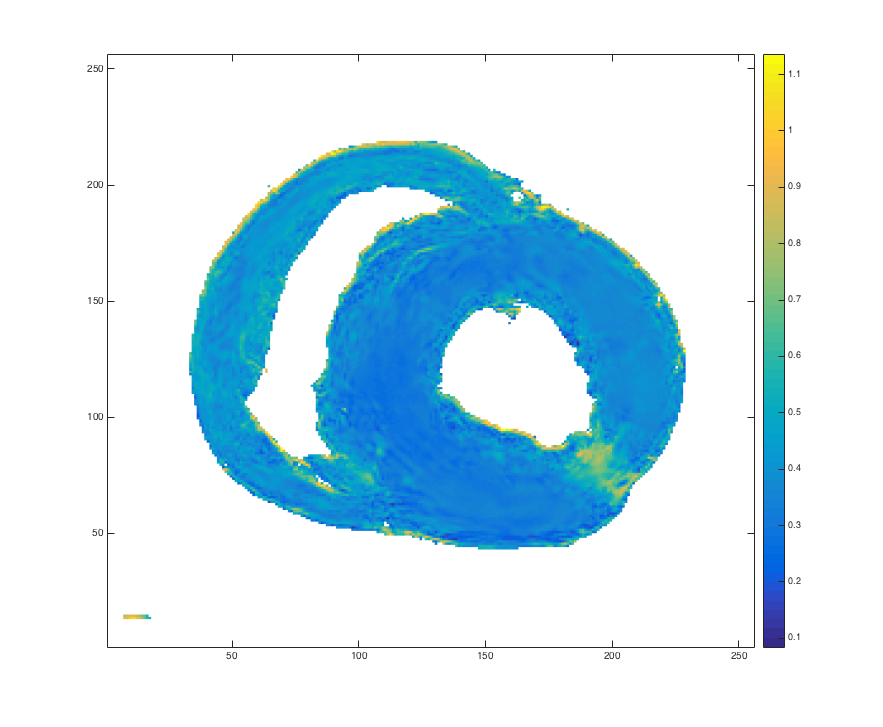
\includegraphics[width=\textwidth]{figures/pig2_adc_31}
        \caption{ADC map}
        \label{fig:pig2_adc}
    \end{subfigure}
    \begin{subfigure}{.31\textwidth}
        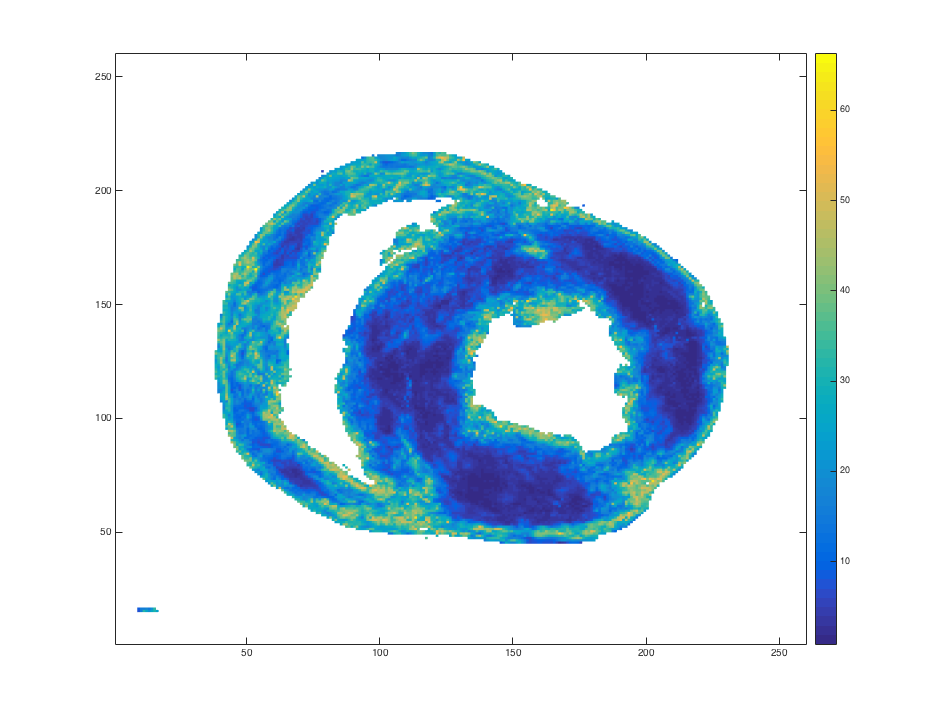
\includegraphics[width=\textwidth]{figures/pig2_err_31}
        \caption{Error of fit}
        \label{fig:pig2_err}
    \end{subfigure}
    \begin{subfigure}{.31\textwidth}
        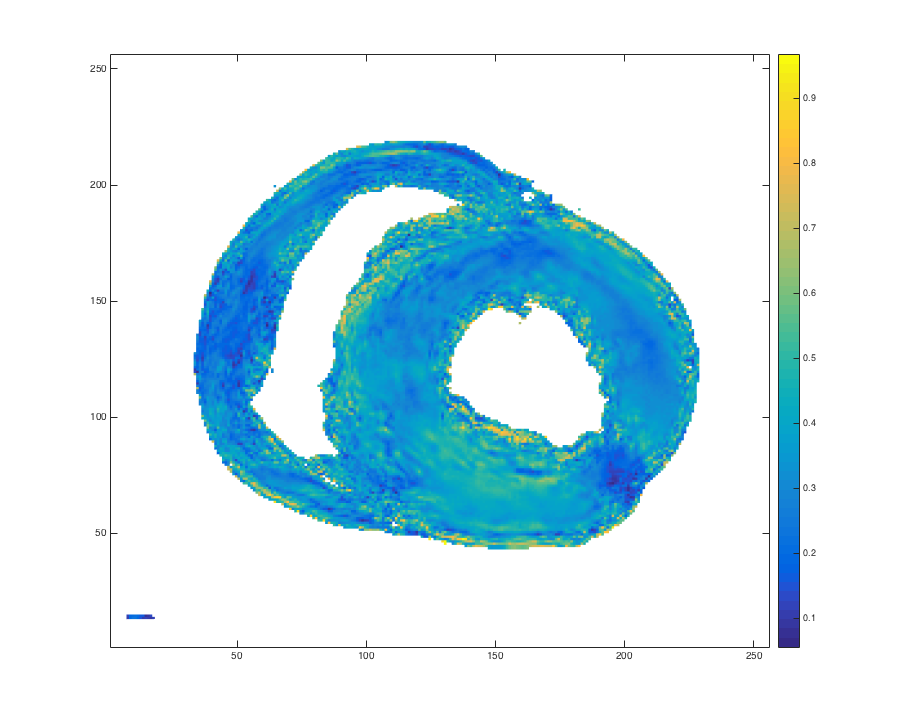
\includegraphics[width=\textwidth]{figures/pig2_fa_31}
        \caption{FA map}
        \label{fig:pig2_fa}
    \end{subfigure}
    \caption{Pig 2: Error of fit computed using our framework compared to ADC and FA map}
    \label{fig:pig2}


    \begin{subfigure}{.31\textwidth}
        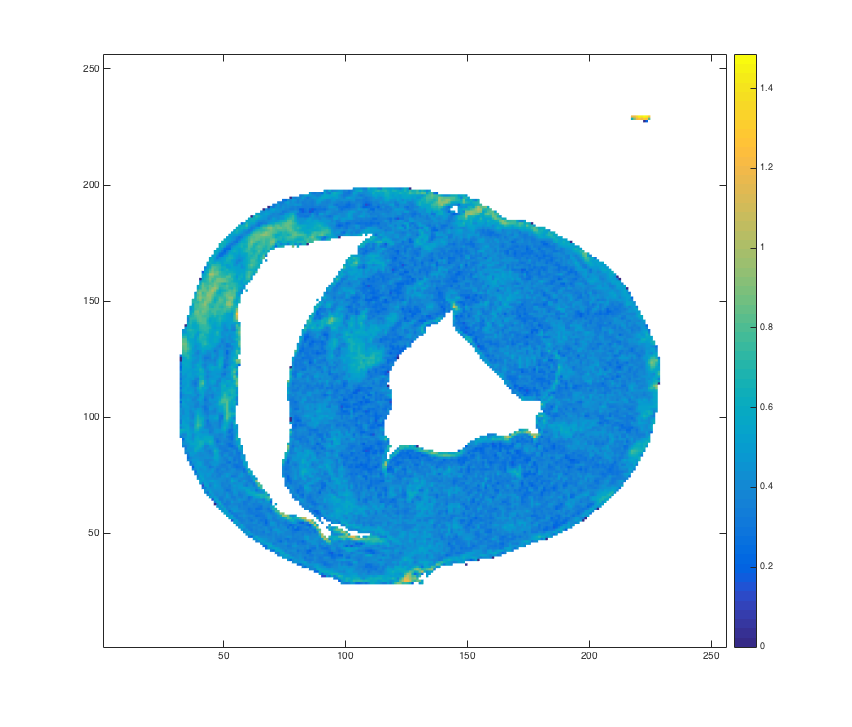
\includegraphics[width=\textwidth]{figures/pig4_adc_21}
        \caption{ADC map}
        \label{fig:pig4_adc}
    \end{subfigure}
    \begin{subfigure}{.31\textwidth}
        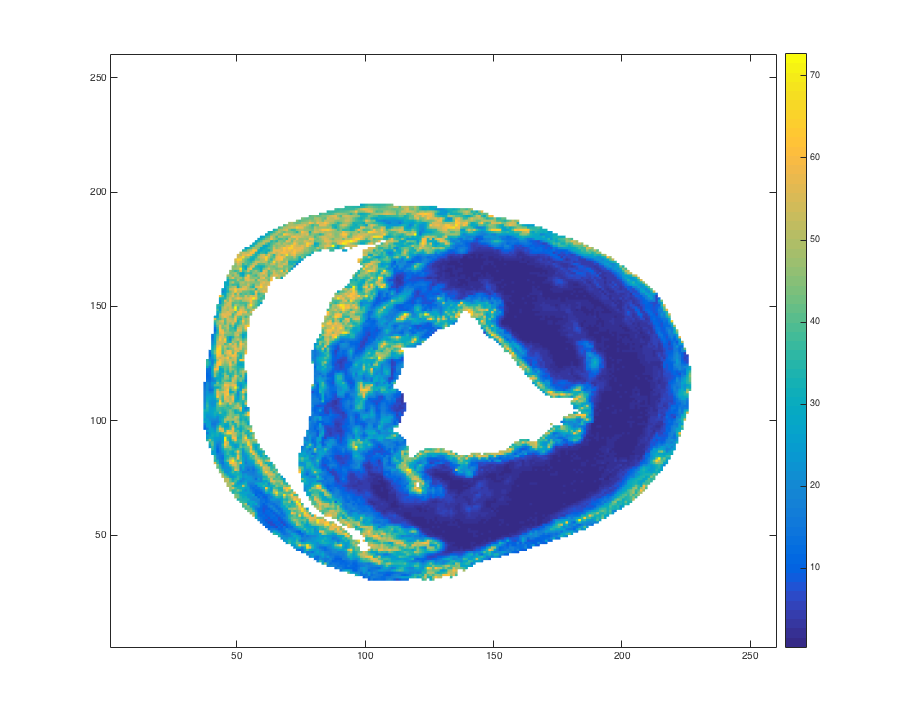
\includegraphics[width=\textwidth]{figures/pig4_err_21}
        \caption{Error of fit}
        \label{fig:pig4_err}
    \end{subfigure}
    \begin{subfigure}{.31\textwidth}
        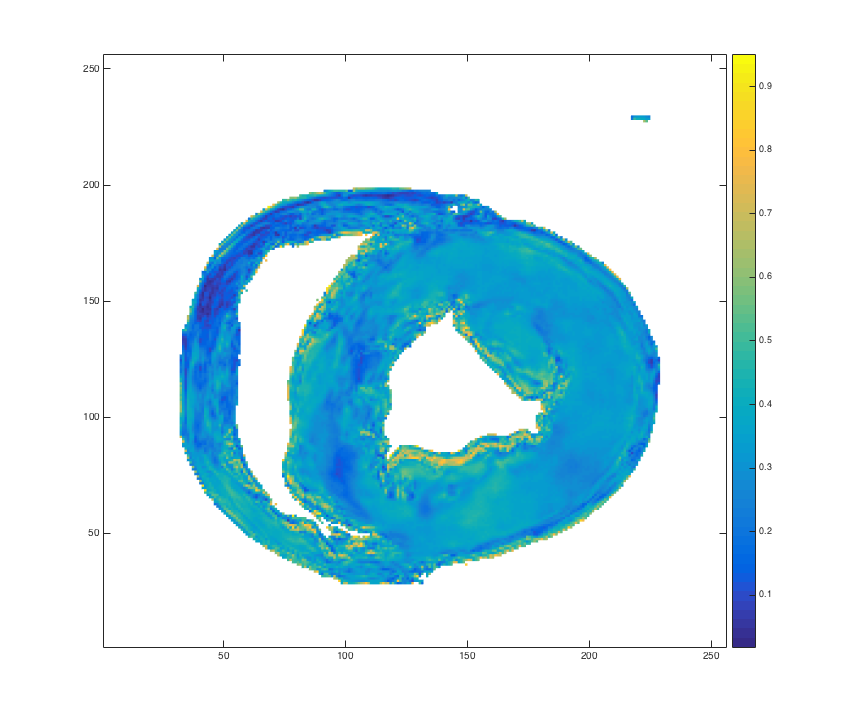
\includegraphics[width=\textwidth]{figures/pig4_fa_21}
        \caption{FA map}
        \label{fig:pig4_fa}
    \end{subfigure}
    \caption{Pig 4}
    \label{fig:pig4}
    
    \begin{subfigure}{.31\textwidth}
        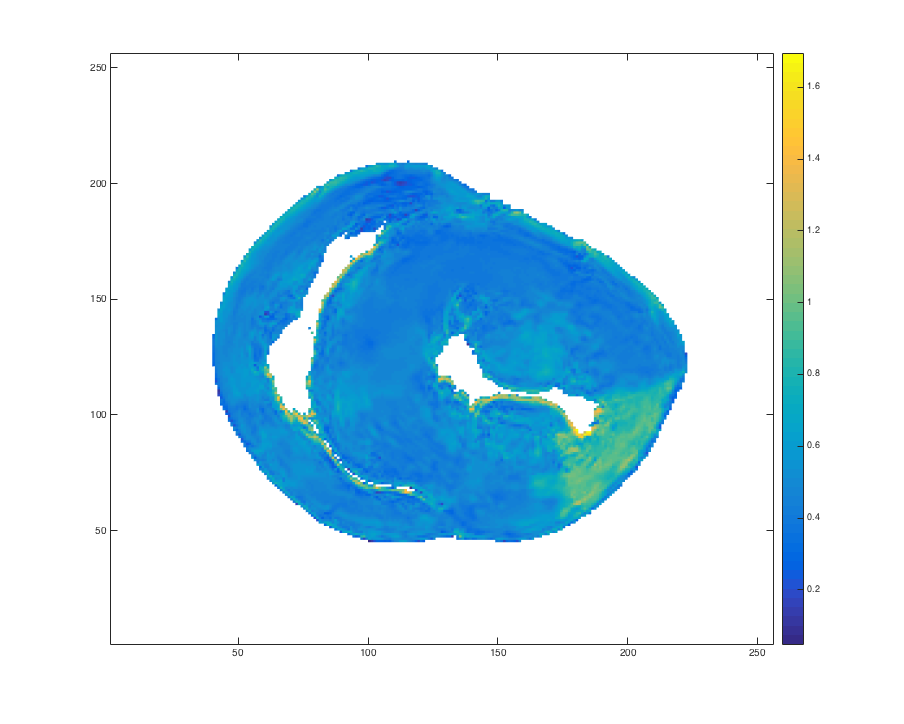
\includegraphics[width=\textwidth]{figures/pig5_adc_22}
        \caption{ADC map}
        \label{fig:pig5_adc}
    \end{subfigure}
    \begin{subfigure}{.31\textwidth}
        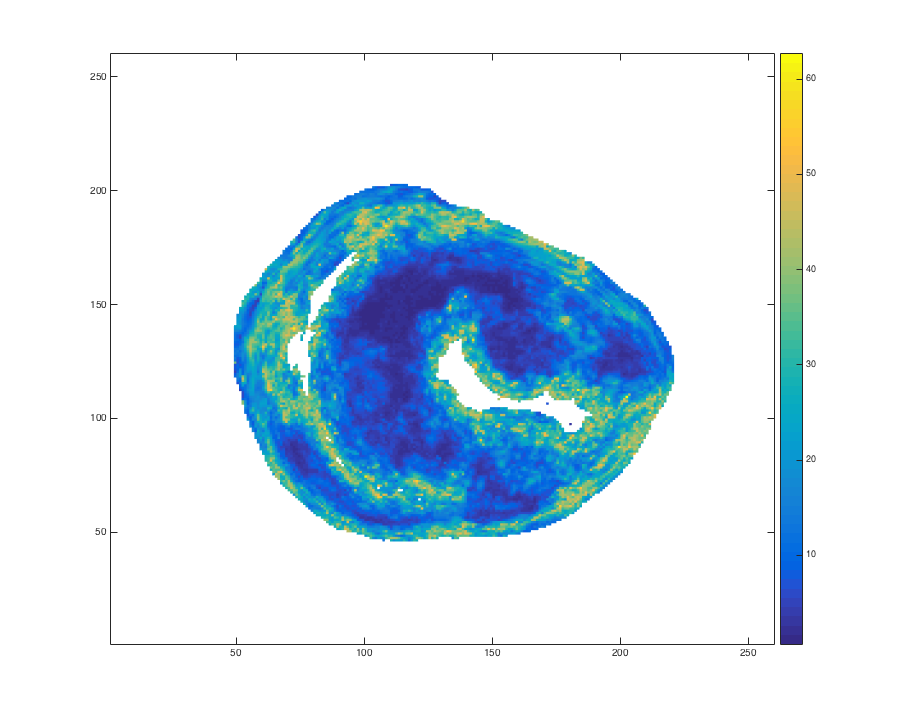
\includegraphics[width=\textwidth]{figures/pig5_err_22}
        \caption{Error of fit}
        \label{fig:pig5_err}
    \end{subfigure}
    \begin{subfigure}{.31\textwidth}
        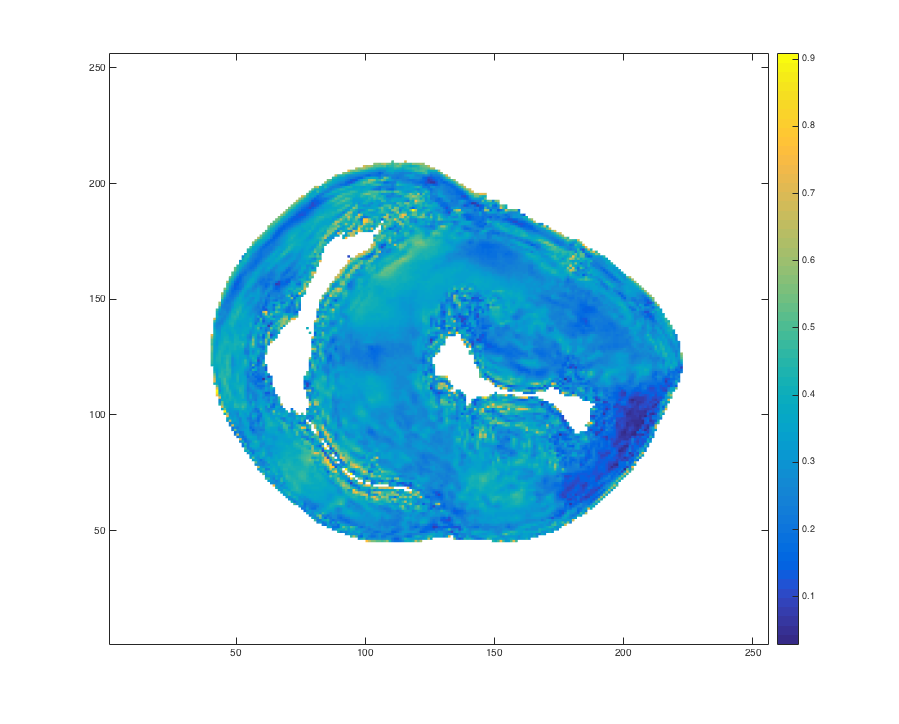
\includegraphics[width=\textwidth]{figures/pig5_fa_22}
        \caption{FA map}
        \label{fig:pig5_fa}
    \end{subfigure}
    \caption{Pig 5}
    \label{fig:pig5}
\end{figure}
    
\begin{figure}
    \centering
    \begin{subfigure}{.31\textwidth}
        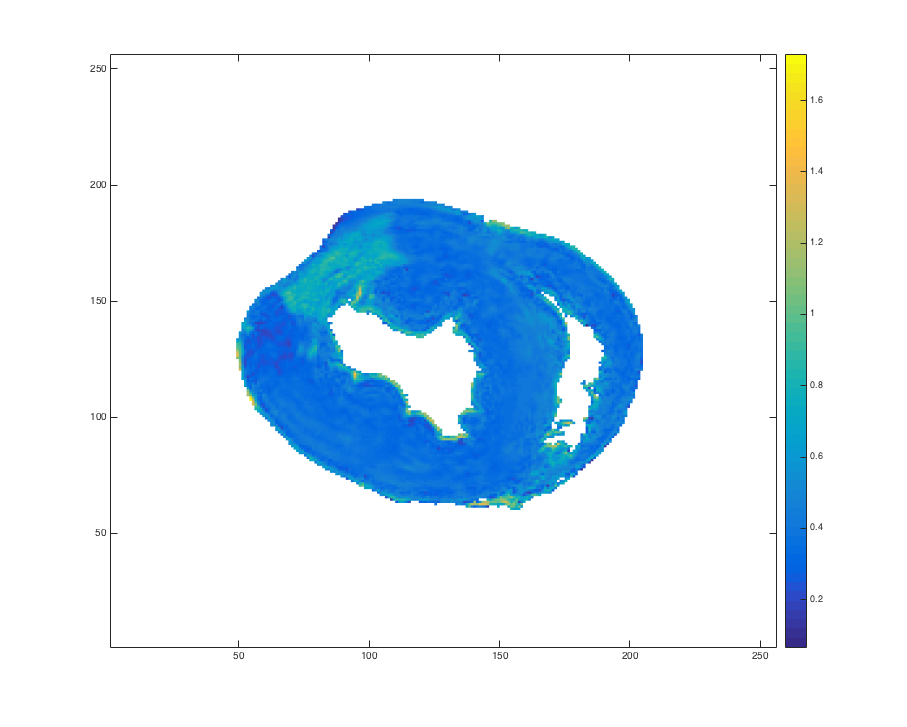
\includegraphics[width=\textwidth]{figures/pig6_adc_24}
        \caption{ADC map}
        \label{fig:pig6_adc}
    \end{subfigure}
    \begin{subfigure}{.31\textwidth}
        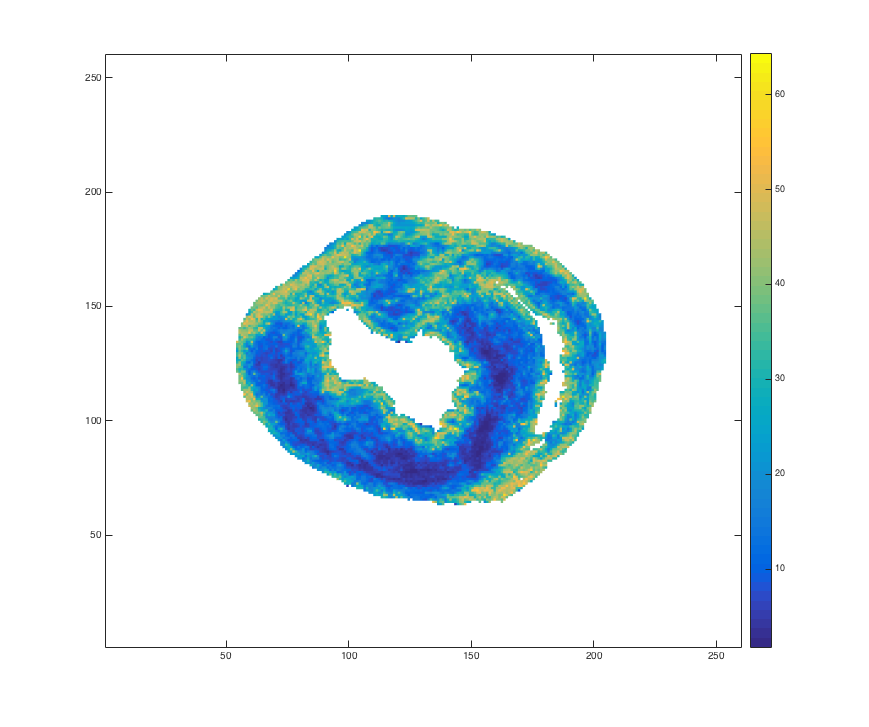
\includegraphics[width=\textwidth]{figures/pig6_err_24}
        \caption{Error of fit}
        \label{fig:pig6_err}
    \end{subfigure}
    \begin{subfigure}{.31\textwidth}
        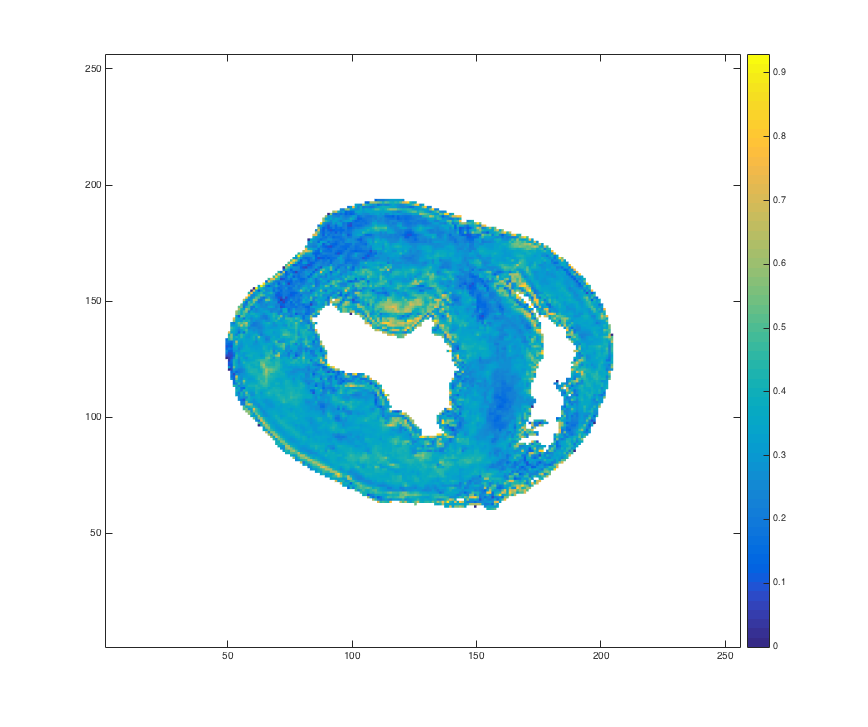
\includegraphics[width=\textwidth]{figures/pig6_fa_24}
        \caption{FA map}
        \label{fig:pig6_fa}
    \end{subfigure}
    \caption{Pig 6}
    \label{fig:pig6}
    
    \begin{subfigure}{.31\textwidth}
        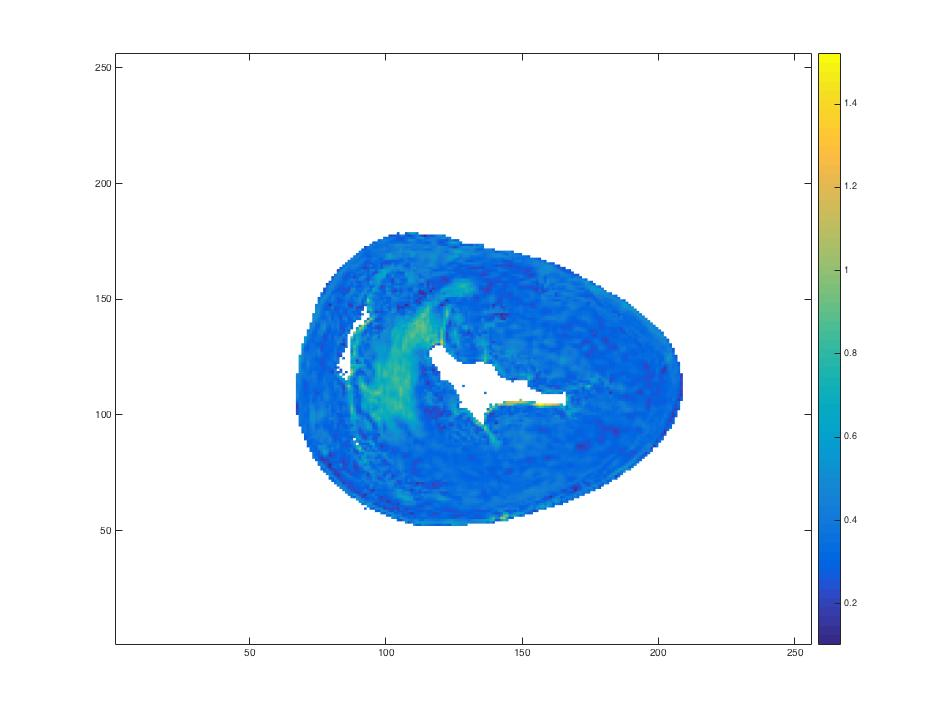
\includegraphics[width=\textwidth]{figures/pig7_adc_14}
        \caption{ADC map}
        \label{fig:pig7_adc}
    \end{subfigure}
    \begin{subfigure}{.31\textwidth}
        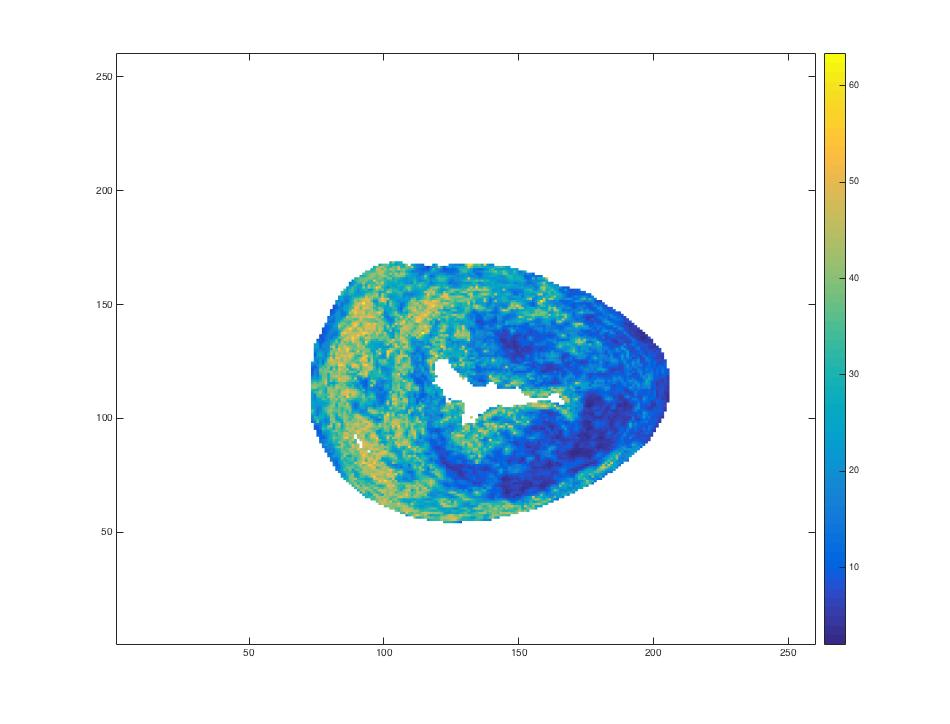
\includegraphics[width=\textwidth]{figures/pig7_err_14}
        \caption{Error of fit}
        \label{fig:pig7_err}
    \end{subfigure}
    \begin{subfigure}{.31\textwidth}
        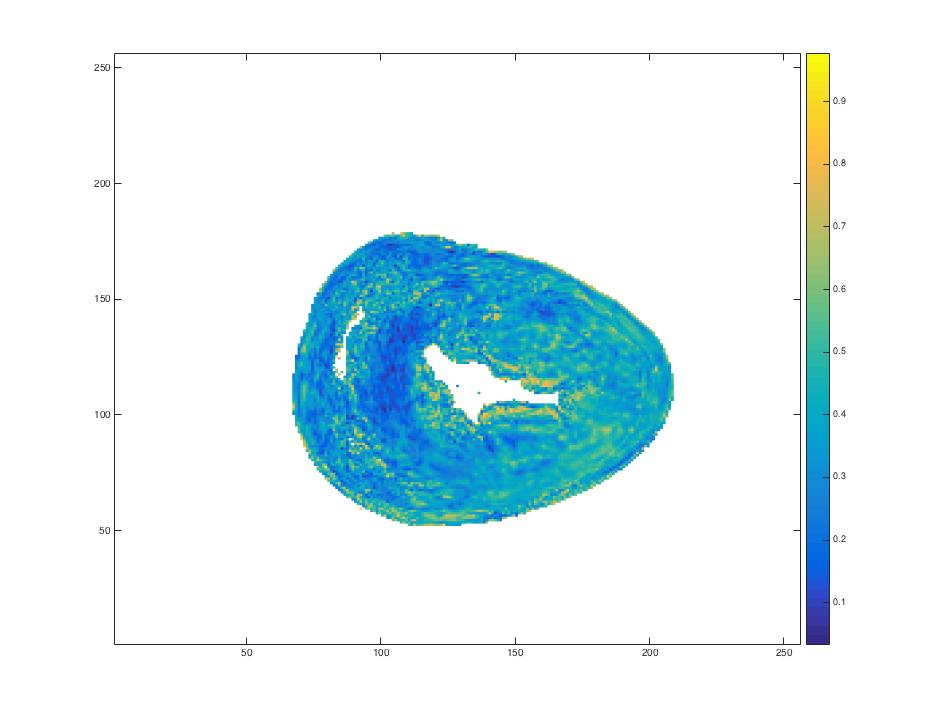
\includegraphics[width=\textwidth]{figures/pig7_fa_14}
        \caption{FA map}
        \label{fig:pig7_fa}
    \end{subfigure}
    \caption{Pig 7}
    \label{fig:pig7}
    
    \begin{subfigure}{.31\textwidth}
        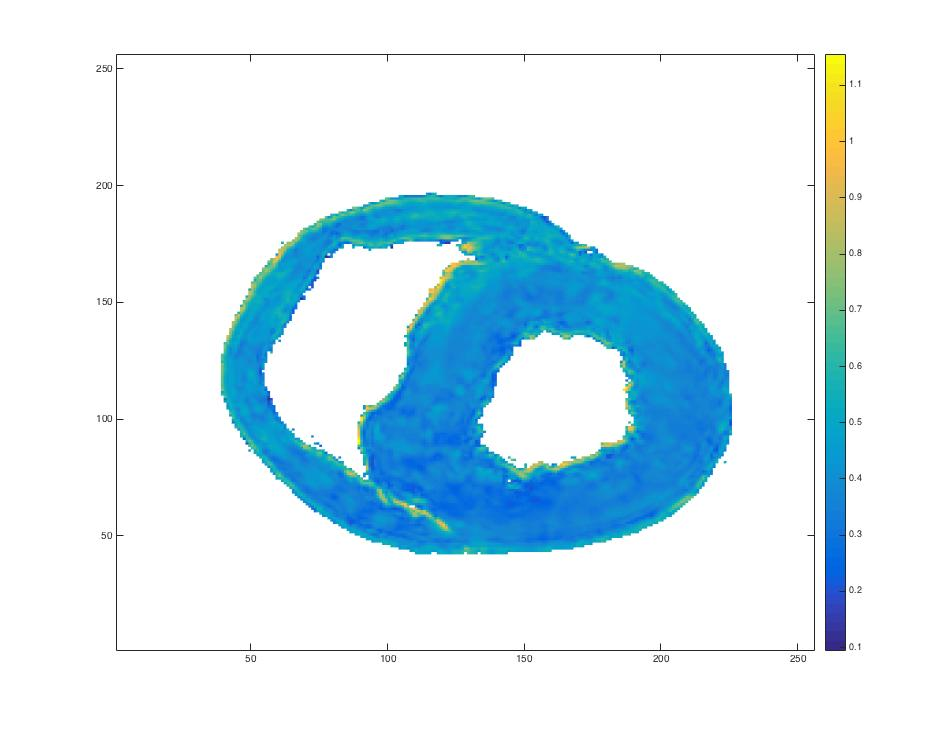
\includegraphics[width=\textwidth]{figures/pig25_adc_30}
        \caption{ADC map}
        \label{fig:pig25_adc}
    \end{subfigure}
    \begin{subfigure}{.31\textwidth}
        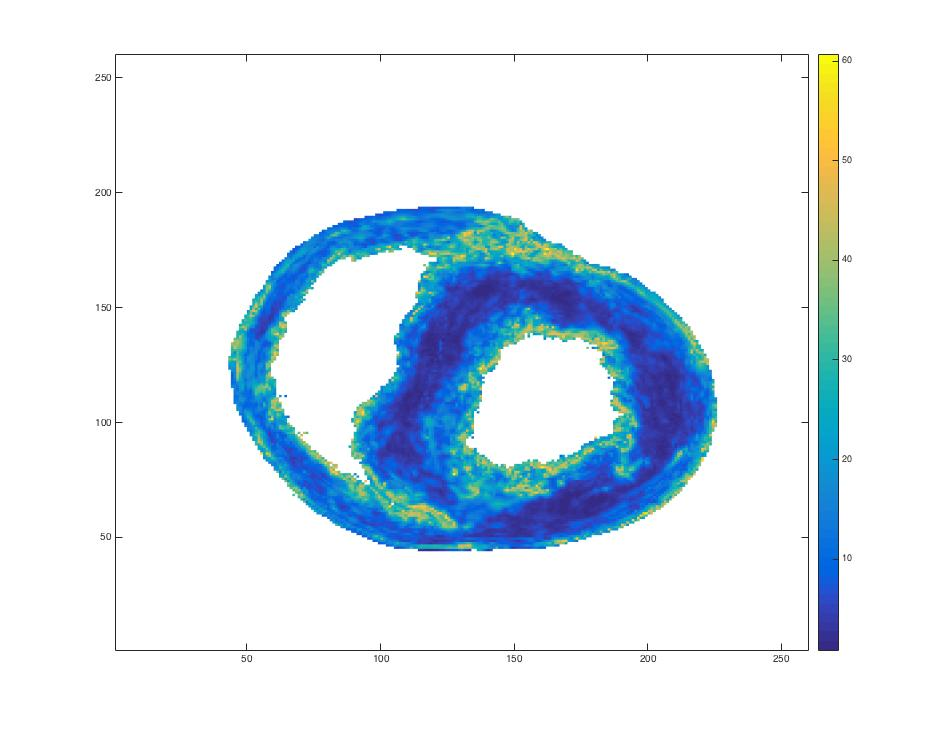
\includegraphics[width=\textwidth]{figures/pig25_err_30}
        \caption{Error of fit}
        \label{fig:pig25_err}
    \end{subfigure}
    \begin{subfigure}{.31\textwidth}
        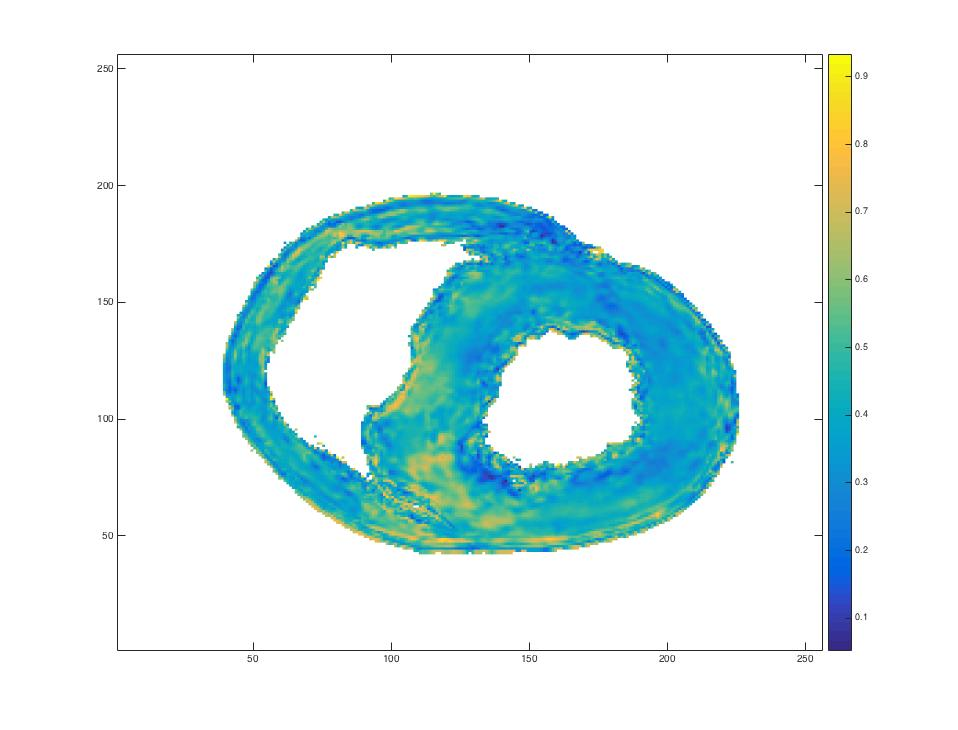
\includegraphics[width=\textwidth]{figures/pig25_fa_30}
        \caption{FA map}
        \label{fig:pig25_fa}
    \end{subfigure}
    \caption{Pig 25}
    \label{fig:pig25}
\end{figure}

Here we get a detailed overview of the data that we worked on to get the presented results. It is clear that the error of fit can provide supplementary information compared to what the ADC and FA scalar maps can give us.

If we focus on the first example - Figure \ref{fig:pig2}, we can see in the ADC map shown in Figure \ref{fig:pig2_adc} the region of the infarct where the value is the highest (yellow region). The FA map goes accordingly. In that precise region there is no observable location where the ADC would be a little bit lower, whereas the error of fit varies more smoothly and shows regions (close to the inner wall for instance) where the error is lower. This region could be a patch of surviving fibers that are still somewhat organized to help the contractile function of the heart. The advantage of the error of fit is that it is more discrete and therefore seems to be more specific in the locations of high error of fits. On the contrary, the FA and ADC maps look more like ink spots that broaden around the infarct region.

This arrangement of the surviving fibers as described in the literature overviewed in Section \ref{surviving_fibers} is also clearly visible in the examples displayed in Figure \ref{fig:pig4} and Figure \ref{fig:pig5}.

The example in Figure \ref{fig:pig6} is also a very interesting sample to compare our method to, and it shows that in some cases as mentioned in \cite{ursell1985structural}, intramural muscles seem to be completely absent in this case. In this case it seems that collagen only is present in the infarct area, with no surviving fibers contributing to wrapping the entire ventricle.

Our approach seems to be more specific and precise in the exhibition of surviving fibers in the infarct region and in some cases show the possible survival of some fibers still contributing to the contractile function of the heart.

The last provided example, Figure \ref{fig:pig25}, is used as a control healthy heart to make sure of the extent to which we can use our results. We can clearly see in this healthy example that the error of fit is low almost everywhere, except in regions near the heart wall (endothilial and epithilial) and the region where the Left Ventricle (LV) and the Right Ventricle (RV) connect to each other. This is due to difficulties in our method to compute connection forms in areas where fibers tend to go in different directions, depending if they work towards the LV contraction, the RV contraction or else. Then the method performs less well to try to fit smoothly varying geometrical fiber structures. Indeed in this case the neighborhood of a fiber can contain fibers wrapping around the LV and fibers wrapping around the RV. These neighbor fibers have a completely different orientation and are responsible for the high error of fit in this region.

\subsection{Discussion}

In all the examples seen in the previous section, locations where the ADC value is high correspond roughly with ones where the error of fit is high. This is to be expected since a high ADC value corresponds to areas with more collagen and less fibrous tissue. The high error of fit is a sign of lack of consistency in the orientation of fibers, which can mean two things. Either the region is less populated in healthy and organized fibers, or the region observed does not contain fibers but other cells that do not have the physical properties of fibers and their geometrical organization.

The error of fit shows additional information that could support existence of surviving fibers in the infarct and border zone that can help the contractile function of the heart after the infarct. This knowledge would be very useful as it is a non-invasive way to qualify the capacity of the heart to keep beating and pumping blood to the body although the heart has suffered from an infarct. Further experiments could be made to support this analysis and show how the efficiency of an infarcted heart is related to the remaining fibers by conducting blood flow experiments before the imaging process.

Another very promising research topic would be to analyze the evolution of surviving fibers at different time frames after infarct, as we were limited to the datasets available which were all 6 weeks after infarct.
